\chapter{Offline Algorithms}

To solve the coverage problem in an optimised fashion the problem was approached as Vehicle Routing Problem, shortly VRP, using a greedy strategy which will be discussed in depth in the next paragraphs. 
The power of this algorithm is that the paths created are cycles so that at the end of the execution all the robots are back in the beginning position, which can be useful from a logistic point of view in a urban search and rescue application, and it's convenient from an energetic point of view. For a survey on \textit{green} VRP see \cite{greenVRP}. To get to the final version of the VRP Greedy I went through some intermediate solutions that I will describe in the following section to show the evolution of algorithm. The first version was just using nearest neighbour nodes when constructing the path, but in a multi-robot approach this turned out to be highly inefficient. So the A* algorithm came in to take into account all the vertices still to be inserted and using the shortest path algorithm to find a way to non-neighbouring vertices. But when increasing the size of the maps computing the A* algorithm each step of the Greedy alg. became time consuming. So finally, since the map is known a priori the Floyd-Warsall algorithm became the most natural solution to find the shortest paths between all pair of vertices at once and this drastically increased the execution time.


%\setcounter{section}{1}
\section{$\min \max$ Vehicle Routing Problem}
\label{s:vrp}

Let's consider the problem of exploring an area with a swarm of quadcopters.


Let $d_{vw}$ be the distance between the vertex $v$ and the vertex $w$.
We can assume that $d_{vw}$ is the euclidean distance between the centre of the cell corresponding to the vertices  $v$ and $w$.
Let $F = \{ 1, \ldots, i, \ldots, N\}$ be the set of quadcopter and let $s_i$ be the starting vertex  of the quadcopter $i$.
A path $P_i$ is assigned to each quadcopter, consisting in an ordered sequence of vertices of $V$ to be visited.
In particular the path of each quadcopter $i$ starts in $s_i$ and ends in $e_i$.
Let $\ell(\cdot)$ be the function that returns the length of a path and, in particular, let $\ell(P_i) \equiv \ell_i$ be the length of the $i-$th path.

The problem consist in planning the trajectories such that:

\begin{enumerate}[label=\textbf{\arabic*.}]
\item the distance travelled by  the quadcopter with the longest path is minimized

\item every vertex is visited at least once
\end{enumerate}

In symbols:
\begin{equation}
\min \quad \mathcal{L} \label{e:obj}
\end{equation}
subject to:
\begin{equation}
\mathcal{L} \geq \ell(P_i) \quad \forall i \in F \label{e:max}
\end{equation}
\begin{equation}
v \in \cup_{i \in F} P_i \quad \forall v \in V \label{e:allIncluded}
\end{equation}


Where \eqref{e:obj} is the \textit{objective function},
the constraints \eqref{e:max} impose $\mathcal{L}$ as maximum length and
the constraints \eqref{e:allIncluded} impose that every node is visited.

\section{The Greedy Algorithm}
\label{s:greedy}
The greedy algorithm is a constructive procedure that iteratively produces a solution.
At each iteration the algorithm takes an incomplete solution (potentially empty) and adds a vertex to produce a new solution.
At every step the algorithm finds the vertex $v$ to be inserted, together with the path $i$ and the position $p$ in which the vertex has to be inserted.

In particular there are two nested levels of optimisation.
The first one is path-local and, for a given robot $i$, checks among the different insertion positions $p$ of a same vertex $v$ which one generates the shortest tentative path length.
The second level of optimisation instead is global and checks among all the shortest $P_i$ paths which one generates the smallest increment with respect to the current longest path. The current length of the longest path will be identified with the letter $\mathcal{L}$.
The choice is made by testing the $\delta_{vip}$ increment in the objective function and then choosing the configuration $<v,i,p>$ that produces the smallest increment.
The complexity of the algorithm is then polynomial $O(\vert V \vert^2 N)$.

In the basic version is convenient to use a single variable $\delta$ and a single triplet \mbox{$<v,i,p>$} to be updated at every iteration. We will call $P_i^{<v,i,p>}$ the path $P_i$ modified inserting the vertex $v$ in the position $p$.
It is convenient, for an implementation point of view, to save the tentative path $P_i^{<v,i,p>}$ in a variable different from $P_i$ (it is enough just a single temporary path instead of one for each vehicle).

\begin{algorithm}[ht]
\begin{algorithmic}[1]
\STATE{$U \leftarrow V$} \label{a:initU}
\FORALL{$i \in F$} \label{a:initFor_i}
\STATE{$P_i \leftarrow \left( s_i, e_i \right) $}\label{a:initP_i}
\ENDFOR \label{a:endForiniti}
\WHILE{$U \neq \emptyset$}\label{a:bigWhile}
\STATE{$(\delta_{vip},\delta^{\text{best}}) \leftarrow + \infty$}\label{a:initDelta}
\STATE{$\mathcal{L} = \max_{\forall i \in F} \ell(P_i)$}\label{a:initBigL}
\STATE{choice $\leftarrow \emptyset$}\label{a:initChoice}
 \FORALL{$v \in U$}\label{a:forV}
  \FORALL{$i \in F$}\label{a:forI}
  \STATE{$(\ell_{i}^{\text{ min}}, \ell_{i}^{\text{ tent}}) \leftarrow + \infty$}\label{a:initLength}
   \FORALL{position $p \in P_i$}\label{a:forPos}
   \STATE{$\ell_{i}^{\text{ tent}} = \ell(P_i^{<v,i,p>})$}\label{a:updateLtent}
    \IF{$\ell_{i}^{\text{ tent}} < \ell_{i}^{\text{ min}}$}\label{a:checkLtent}
    \STATE{$\ell_{i}^{\text{ min}} = \ell_{i}^{\text{ tent}}$}\label{a:updateLmin}
    \STATE{$\delta_{vip} = \ell_{i}^{\text{ min}} - \mathcal{L}$}\label{a:calcDelta}
    \IF{$\delta_{vip} < \delta^{\text{best}}$}\label{a:testDelta}
     \STATE{$\delta^{\text{best}} \leftarrow \delta_{vip}$}\label{a:saveDelta}
     \STATE{choice $\leftarrow <v,i,p>$}\label{a:saveChoice}
    \ENDIF \label{a:endIfTestDelta}
    \ENDIF
   \ENDFOR \label{a:endForPos}
  \ENDFOR \label{a:endForI}
 \ENDFOR \label{a:endForV}
 \STATE{add $v$ to $P_i$ in position $p$} \label{a:doIt}
 \STATE{$U \leftarrow U \setminus choice.v$}  \label{a:removeV}
\ENDWHILE \label{a:endBigWhile} 
\RETURN{$P = \cup_{i \in F}P_i$} \label{a:return}
\end{algorithmic}
\caption{Greedy algorithm for the $\min \max$ VRP}\label{alg:greedy}
\end{algorithm}

Here is the algorithm in detail:
the rows \ref{a:initU}--\ref{a:initChoice} are used to initialise all the variables.
In particular the structure of $U$ is initialised (line \ref{a:initU}) with the set of all  the accessible nodes (not shown in the code: the start nodes $s_i$ are excluded).
The paths are initialised with a sequence that begins and ends with the starting nodes  (\ref{a:initFor_i}--\ref{a:endForiniti}). 
At the beginning of the main loop (line \ref{a:bigWhile}),
the variable $\delta_{vip}$, containing the increments of the objective function is initialised at plus infinite, and the same thing goes for the best increment $\delta^{\text{best}}$ (line \ref{a:initDelta}).
We then initialise $\mathcal{L}$, with the length of the longest path and reset the best choice (lines \ref{a:initBigL}--\ref{a:initChoice}).
In the next three nested loops (lines \ref{a:forV}--\ref{a:endForV}) is tested the insertion of every vertex $v \in U$ in every possible position $p$ of every possible path $i$. For a given robot $i$, the length after the insertion, called $\ell_{i}^{\text{ tent}}$, is then compared to the smallest current length among all the insertions,  $\ell_{i}^{\text{ min}}$ (line \ref{a:checkLtent}).
Note: the position to consider are the ones included between the position after the start and before the end. If the tentative length is smaller than the current best one it becomes the new best (line \ref{a:updateLmin}) and the increment is calculated with respect to the objective function previously evaluated, using the following formula:
\begin{equation}\label{e:delta}
\delta_{vip} = l_{i}^{\text{ min}} - \mathcal{L}
\end{equation}
The best $<v,i,p>$ triplet (line \ref{a:testDelta}) is saved (line \ref{a:saveChoice}) together with the corresponding increment (line \ref{a:saveDelta}).
After all the for loops are executed the best insertion is applied (line \ref{a:doIt}) and the chosen vertex is removed from the list of unvisited vertices (line \ref{a:removeV}).
When the unvisited set $U$ is empty (line \ref{a:endBigWhile}), the solution is returned (line \ref{a:return}).





\section{VRP Greedy Nearest Neighbour}

This version of the VRP Greedy follows basically the exact same scheme explained in the previous paragraph. The reason why it was called the ``Nearest Neighbour'' comes from the way it looks for the vertices. The candidates vertices to be inserted in a the path of a robot $i$ are chosen among all the vertices in the neighbouring of that robot's path $P_i$. Remember that by how we defined our graph in the first chapter (\ref{sec:terminology}), a vertex $v$ has edges that point only to its neighbours $w_i$, so any other vertex insertion would have been inconsistent. So if we are to test vertex $v_t$ in positon $p$ of path $P$ we only insert it if $e(P(p-1),v_t)=1$ and $e(P(p-1),v_t)=1$.
If we were to operate with a single robot, it always true that there exist a neighbour unvisited vertex, but this is no more valid when we deal with a swarm of robots. To solve this problem the VRP Greedy A* was developed.

\section{VRP Greedy A*}

This extension of the previous VRP make possible for the algorithm to check vertices which are not in the neighbouring of a certain $P_i$ path. When all the neighbour vertices of a certain path have been already visited, the greedy search starts looking for all the remaining vertices, and it finds a way through the graph using the A* path-finding algorithm. In particular if we consider the insertion of a vertex $v$ in a position $p$, the destination position will be between the vertex $P(p)$ and $P(p-1)$. The algorithm checks firstly whether the vertex $v$ is a neighbour of $P(p-1)$ and, if not, it calculates the so called ``\emph{way there}''. Then it checks whether the vertex $v$ is a neighbour of $P(p)$ and, if not, it calculates the so called ``\emph{way back}''. The final A* path will be then:

\begin{equation}
way there + v + way back \label{e:astarpath}
\end{equation}

To fit the behaviour of this algorithm the \mbox{$<v,i,p>$} variable was modified by introducing a fourth parameter $n$, a boolean variable which tells if the current best choice is a vertex adjacent to the corresponding $P_i$ path or not. The resulting new choice was simply called \mbox{$<v,i,p,n>$}, and a the moment of the insertion (line \ref{a:doIt} of algorithm \ref{alg:greedy}), if $n=\texttt{false}$ the A* path of will be inserted in position $i$.

The problem found with this approach was that the A* algorithm is performed every time a vertex $v$ is tested on a position $p$ and since the greedy algorithm tests all the possible configuration, on maps with more than 100 nodes the computational time started to be too big. Moreover if assume the map is not changing, which we are, there is no need of computing the shortest path every time, and that's why the next algorithm was developed.


\section{VRP Greedy with Floyd-Warshall}

The Floyd-Warshall algorithm is a method to find the lengths of the paths between all pairs of vertices. Using an auxiliary \textit{parent} structure it also possible to to get the actual path, needed for the final evaluation of the optimal coverage path. The Floyd-Warshall algorithm falls in the category of \textit{dynamic programming} since it breaks down the problem of finding a path between two arbitrarily distant vertices into simpler sub-problems.

The algorithm maintains a distance matrix ($D$) such that at iteration $k$, $d_{ij}$ is the shortest path from $i$ to $j$ using nodes 1, 2, ...$k$ as intermediate nodes. After the algorithm terminates, assuming that no negative cost cycle is present, the shortest path from nodes $i$ to $j$ is $d_{ij}$. $P$ is the parent matrix, and the meaning of its entries $p_{ij}$ is: ``for some shortest path from $i$to $j$, the vertex right before $j$ is $p_{ij}$". So given a graph $G(E,V)$, the algorithm proceeds as follows:

\begin{algorithm}[ht]
\begin{algorithmic}[1]

\STATE{$D \leftarrow G$} \label{fw_initD}
\STATE{$P \leftarrow G$} \label{fw_initP}
\FORALL{$i \in G$} \label{fw_initFor_i1}
  \FORALL{$j \in G$} \label{fw_initFor_j1}
    \relax
    \IF {$i == j \lor d_{ij} == \infty$}
    \STATE {$p_{ij} = -1$}
    \ELSE
    \STATE {$p_{ij} = i$}
    \ENDIF
  \ENDFOR
\ENDFOR
\FORALL{$i \in G$} \label{fw_initFor_i2}
      \FORALL{$j \in G$} \label{fw_initFor_j2}
	  \FORALL{$k \in G$} \label{fw_initFor_k2}
	   \STATE {$dist_{ikj} = d_{ik} +d_{kj}$}
	    \IF {$dist_{ikj} < d_{ij}$}
	    \STATE {$d_{ij} =dist_{ikj} $}
              \STATE {$p_{ij} = p_{kj}$}
	    \ENDIF
	  \ENDFOR
      \ENDFOR
\ENDFOR
\RETURN{$D$} \label{a:return_D}
\end{algorithmic}
\caption{Floyd-Warshall Algorithm}\label{alg:floydWarsh}
\end{algorithm}

We initialize all entries $p_{ij}$  to $i$ when we have an edge, and if not we set it to $-1$. The update process of the parent array basically mean the following: ``if going from $i$ to $j$ through $k$ ($i \rightarrow k \rightarrow j$) is an improvement, then we set the parent of $j$ in the new shortest path to the parent of the path $k  \rightarrow j$". To recover the path from $i$ to $j$ simply recurse on $p_{ij}$'s entries.
In this formulation inside the triple loop of the greedy solver the vertices inserted in the path are just the one in the unvisited set $U$, without all the shortest paths between not adjacent nodes. The shortest paths all inserted all at once at the end of the execution (post-insertion), and not while executing the solver (contextual-insertion). This reduces a lot the number of possible insertion positions $p \in P_i$ increasing the algorithm execution speed, but also meaning that we reduce the amount of solution space we explore. Some comparisons between result with the shortest path contextual-insertion and the post-insertion showed that there was so significant improvement to justify the former approach in favour of the latter.

In the next chapter will be presented the results obtained for the different algorithms and due to the motivation explained in this chapter the only algorithm used for the offline class will be the VRP Greedy using Floyd-Warshall.
\pagebreak

\section{Implementation}

In this case the paths are preprocessed and the robots are guided by a central ROS node which compute the optimal path. The central node is called \emph{kernelNode} and as it can be seen in Fig. \ref{fig:nonrt_nodes} it communicates with all the quadcopter controllers through two topics: \emph{quadCtrlSignal} and \emph{pathCompleted}. Same as the before all the nodes are launched together using the \texttt{roslaunch} package, but the \emph{quadcopterRosCtrl} nodes are not able to publish their position commands until the \emph{kernelNode} is done computing the paths. Only then the central node triggers the ``start'' command, and the control nodes start moving the quadcopters. When a quadcopter finishes to follow its path, it publish a message over the \emph{pathCompleted} topic. When all the quadcopters are done, the central node stops triggering the control signal and the ROS network is shut down.


\begin{figure}[h]
\centering
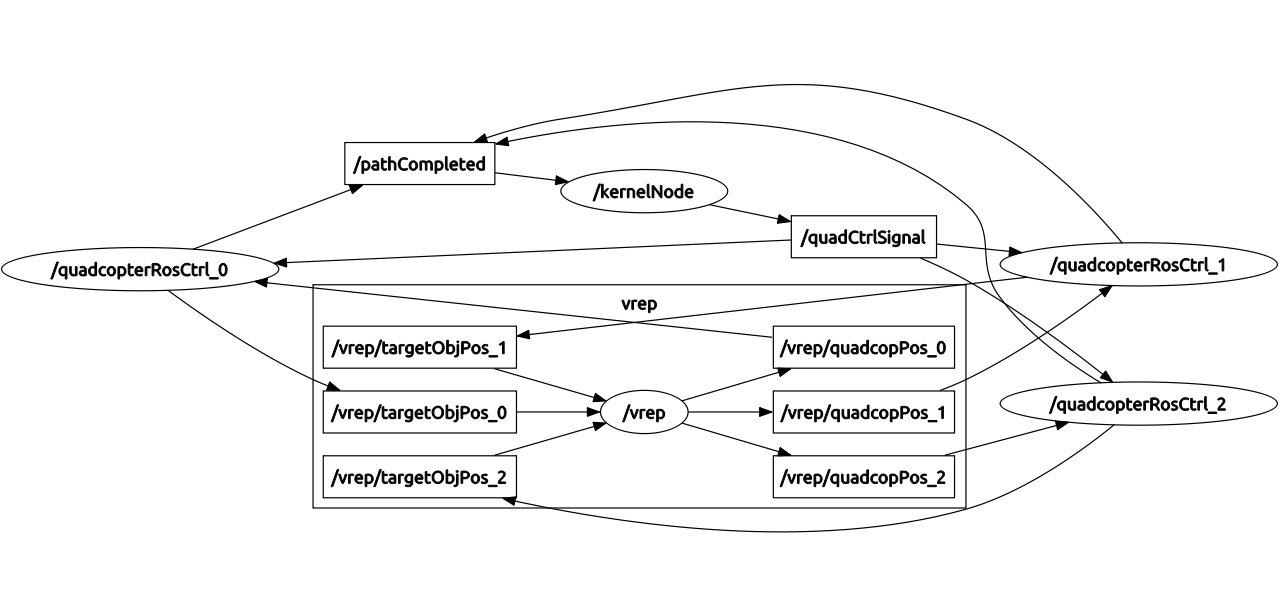
\includegraphics[scale=0.3]{swarm_Greedy}
\caption[ROS network for the offline algorithms]{The nodes and topics ROS network of the offline algorithms. The ellipses are nodes while the rectangles are topics.}
\label{fig:nonrt_nodes}
\end{figure}



